\section{Results}
\label{sec:results}

Unless stated otherwise, predictive results come from the single locked final test (545 students,
213 dropouts), whereas the explanation-audit and sensitivity results use only the 544 validation
students and are post-hoc.

\subsection{Predictive Performance on the Locked Final Test}
\label{sec:perf}

Table~\ref{tab:final-test} and Figure~\ref{fig:final-test} summarise the five models. \tabicl
achieved the highest point ROC-AUC (0.957), although XGBoost (0.956), EBM (0.954) and logistic
regression (0.953) were all within 0.004. At the fixed capacity, the five models flagged between
107 and 109 of the 213 dropouts. \tabicl flagged 109 students, of whom 108 dropped out (precision
0.991), and identified 108 of the 213 dropouts (recall 0.507); its confusion matrix was TN\,=\,331,
FP\,=\,1, FN\,=\,105 and TP\,=\,108. XGBoost achieved the best Brier score and calibration, while EBM
achieved the best capacity recall and precision.

\begin{table}[!htb]
\centering
\caption{Locked final-test results (545 students, top 20\% flagged; best in bold).}
\label{tab:final-test}
\footnotesize
\setlength{\tabcolsep}{3pt}
\begin{tabular}{@{}lccccc@{}}
\toprule
\textbf{Model} & \textbf{AUC} & \textbf{Brier} & \textbf{ECE} & \textbf{Rec.@20\%} & \textbf{Prec.@20\%} \\
\midrule
Logistic reg. & 0.9525 & 0.0822 & 0.066 & 0.507 & 0.991 \\
Decision tree & 0.9099 & 0.0999 & 0.069 & 0.502 & 0.982 \\
XGBoost       & 0.9557 & \textbf{0.0711} & \textbf{0.029} & 0.507 & 0.991 \\
EBM           & 0.9539 & 0.0768 & 0.040 & \textbf{0.512} & \textbf{1.000} \\
\tabicl       & \textbf{0.9566} & 0.0740 & 0.032 & 0.507 & 0.991 \\
\bottomrule
\end{tabular}
\end{table}

\begin{figure}[!htb]
  \centering
  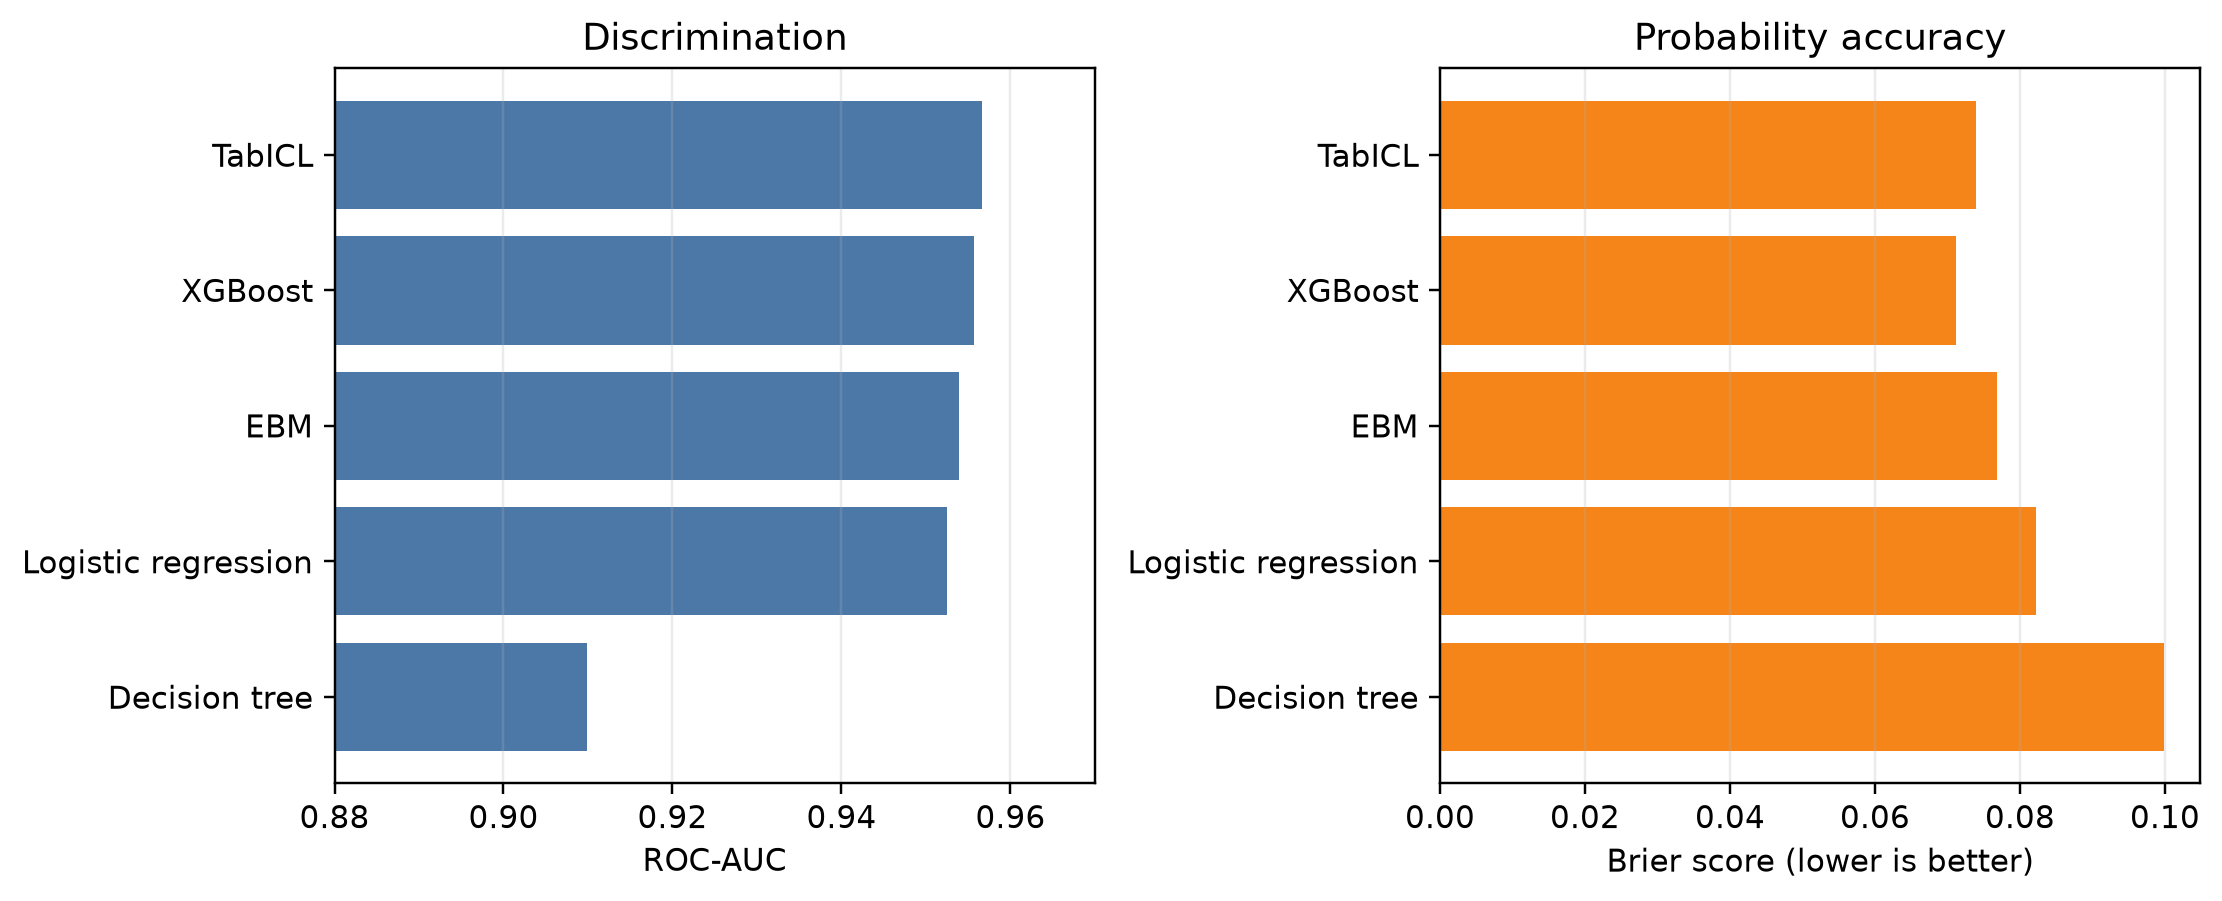
\includegraphics[width=\linewidth]{final_test_model_performance.png}
  \caption{Final-test ROC-AUC and Brier score for the five models.}
  \label{fig:final-test}
\end{figure}

The paired bootstrap intervals (Table~\ref{tab:paired}) show that \tabicl clearly outperformed the
depth-3 tree but could not be distinguished from XGBoost, EBM or logistic regression, as every
interval for these comparisons includes zero. The answer to RQ1 is therefore that \tabicl adds no
demonstrated predictive value over simpler models on this task.

\begin{table}[!htb]
\centering
\caption{\tabicl minus each baseline on the final test (95\% paired-bootstrap intervals; negative $\Delta$ Brier favours \tabicl).}
\label{tab:paired}
\footnotesize
\setlength{\tabcolsep}{3pt}
\begin{tabular}{@{}lcc@{}}
\toprule
\textbf{Comparison} & \textbf{$\Delta$ ROC-AUC} & \textbf{$\Delta$ Brier} \\
\midrule
vs.\ logistic reg. & 0.004 [$-$0.005, 0.014] & $-$0.008 [$-$0.017, 0.001] \\
vs.\ decision tree & 0.047 [0.029, 0.067] & $-$0.026 [$-$0.036, $-$0.016] \\
vs.\ XGBoost       & 0.001 [$-$0.006, 0.009] & 0.003 [$-$0.003, 0.009] \\
vs.\ EBM           & 0.003 [$-$0.007, 0.014] & $-$0.003 [$-$0.010, 0.004] \\
\bottomrule
\end{tabular}
\end{table}

\subsection{Why Precision Is Nearly Perfect: Who Gets Flagged}
\label{sec:who}

A precision of 0.99 to 1.00 warrants scrutiny rather than celebration. On the validation split,
\tabicl flagged 108 students, all of whom dropped out, and Table~\ref{tab:who} characterises them:
78 passed no first-semester units and 25 took no evaluations at all, while 19 of the 30 who passed
at least one unit had unpaid tuition fees. A one-line rule, ``flag students who passed zero
units'', selects 103 students with a precision of 0.874 and a recall of 0.423, compared with 1.000
and 0.507 for the model. On validation, the model's added value is therefore narrow: it excludes 25
zero-pass students (13 of whom graduated) and adds 30 students with some passed units, most of whom
had fee problems. For most flagged students, therefore, an adviser would learn little beyond what the
transcript already shows, and the flags arrive when these students may already have disengaged.

\begin{table}[!htb]
\centering
\caption{The 108 flagged validation students compared with a simple rule.}
\label{tab:who}
\footnotesize
\begin{tabular}{@{}lr@{}}
\toprule
\textbf{Measure} & \textbf{Value} \\
\midrule
Flagged students who dropped out & 108 / 108 \\
Passed zero first-semester units & 78 \\
Took no evaluations at all & 25 \\
Passed $\geq$1 unit, tuition fees unpaid & 19 of 30 \\
Top explanation is first-semester progress & 108 / 108 \\
\midrule
Rule ``passed zero units'': selected & 103 \\
\quad precision / recall & 0.874 / 0.423 \\
\tabicl at 20\%: precision / recall & 1.000 / 0.507 \\
\bottomrule
\end{tabular}
\end{table}

\subsection{Calibration and Subgroup Diagnostics}
\label{sec:fairness}

Calibration error was small for all models except logistic regression and the decision tree
(Table~\ref{tab:final-test}). Subgroup results on the final test are descriptive, and metrics are
suppressed for groups of fewer than 30 students (all non-Portuguese nationalities, international
students and students with special educational needs). Flag rates differed by gender (0.122 for
group~0, female in the UCI coding, vs.\ 0.324 for group~1, male), displacement (0.136 for displaced
vs.\ 0.288 for non-displaced students) and age (0.116 for students aged 20 or younger vs.\ 0.434 for
ages 26--35). These differences largely follow the dropout base rates (0.30 vs.\ 0.54 by gender);
however, recall also differed, at 0.410 vs.\ 0.593 by gender, 0.414 vs.\ 0.596 by displacement and
0.411 vs.\ 0.655 between the youngest and the 26--35 age bands. The model thus identifies a smaller
share of dropouts among younger, female and displaced students (Appendix Table~\ref{tab:subgroups}).
Furthermore, several non-protected features act as strong proxies for protected attributes:
application route is associated with international status (Cram\'er's $V=0.61$) and age (0.50), and
course with gender (0.40). The model's own leading inputs carry the same signal more weakly: on the
final test, first-semester pass rate is associated with gender ($\eta=0.28$) and age (0.24), and fee
status with age ($V=0.23$). Parental and financial fields may also encode socio-economic
disadvantage. Removing protected columns therefore cannot remove their information.

\subsection{Explanation Faithfulness and Stability}
\label{sec:audit}

\textbf{Faithfulness.} Removing groups in SHAP order changed the prediction far more than removing
them in random order: the mean area between the curves was 1.557 (95\% interval 1.476--1.643) and was
positive for 536 of 544 students (Appendix Figure~\ref{fig:faithfulness}). The explanations
therefore point to information the model actually uses.

\textbf{Content of the explanations.} First-semester progress dominated (mean absolute grouped SHAP
0.277, in the top five for 97\% of students), followed by participation (0.053), tuition fees
(0.051) and course (0.042) (Figure~\ref{fig:top-groups}). As first-semester progress was the
leading reason for every flagged student, the explanation largely restates the transcript precisely
for the students who matter most. Figure~\ref{fig:card} illustrates how such an explanation could
reach a support officer: a flagged validation student who sat ten evaluations but passed no unit,
whose progress bar outweighs every other reason. Global methods agree
(Appendix~\ref{sec:app-pred}).

\begin{figure*}[t]
  \centering
  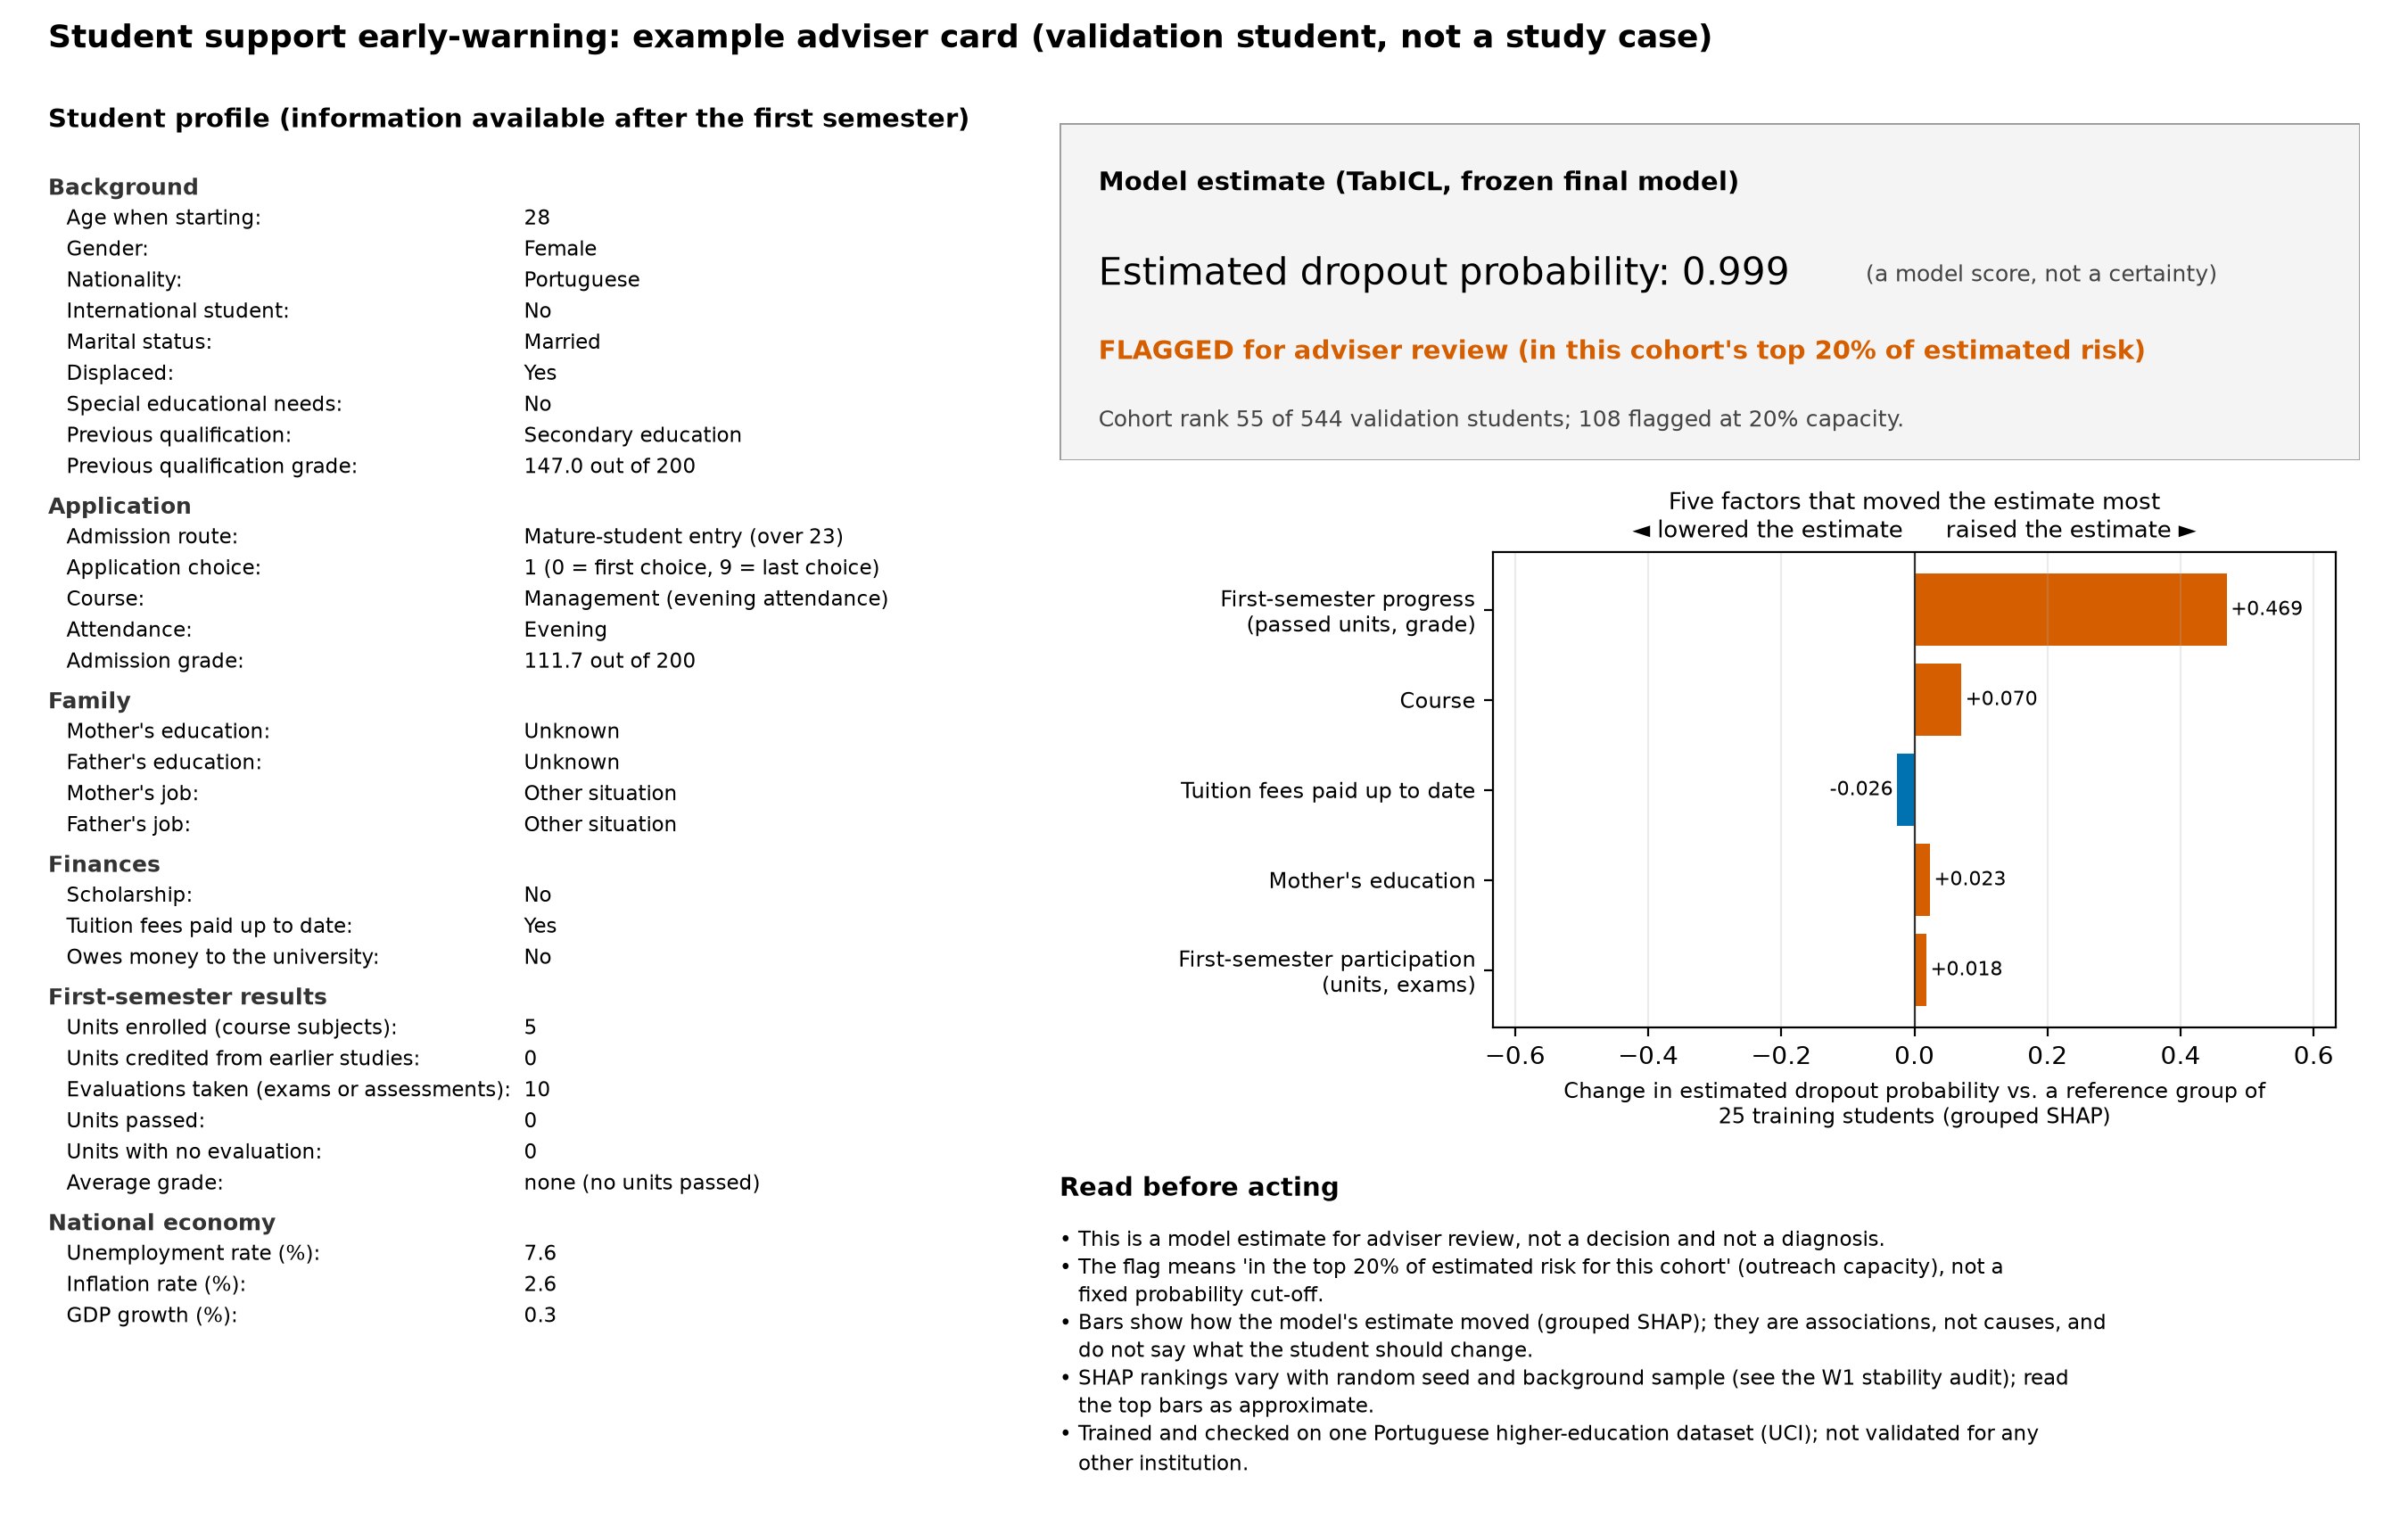
\includegraphics[width=0.62\linewidth]{demo_card_validation.png}
  \caption{Example adviser card for a validation student: the record (left) and the flag, rank and five largest grouped SHAP reasons (right).}
  \label{fig:card}
\end{figure*}

\begin{figure}[!htb]
  \centering
  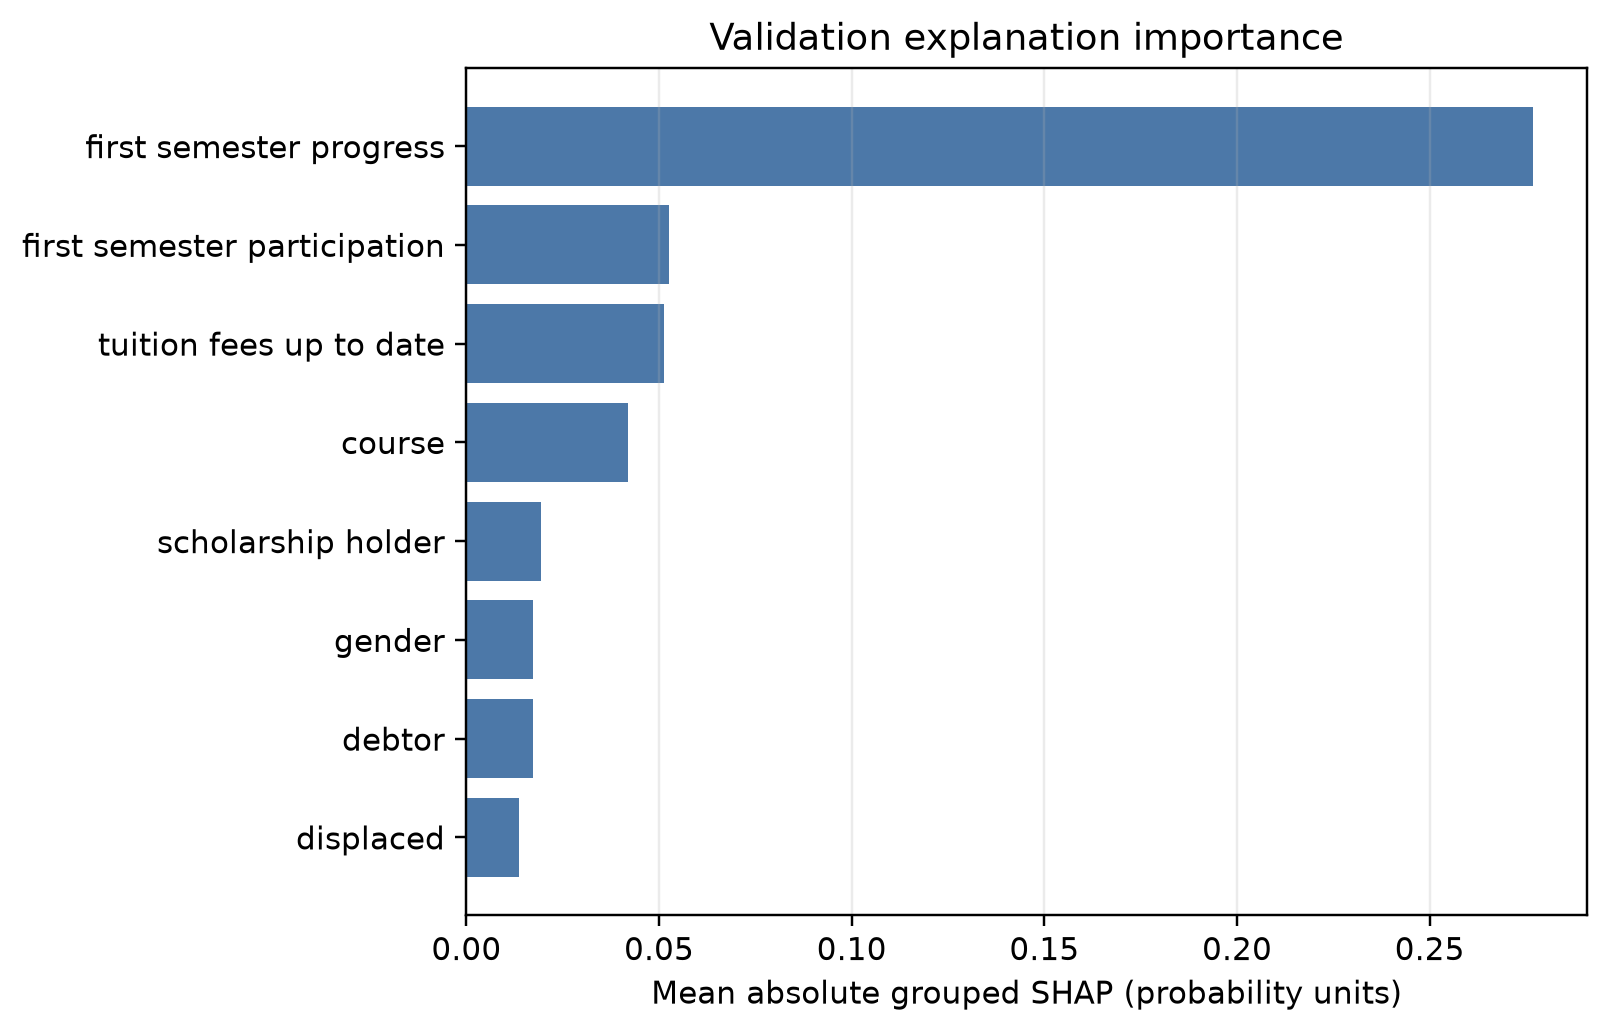
\includegraphics[width=\linewidth]{top_explanation_groups.png}
  \caption{Mean absolute grouped SHAP contribution (544 validation students).}
  \label{fig:top-groups}
\end{figure}

\textbf{Stability.} The ranking of reasons was robust to minimal grade changes (mean top-five
overlap 0.996; no student below 0.80) but not to the explainer's own randomness: overlap was 0.818
across random seeds (213 students below 0.80) and 0.745 across background samples (411 students
below 0.80) (Figure~\ref{fig:stability}).

\begin{figure}[!htb]
  \centering
  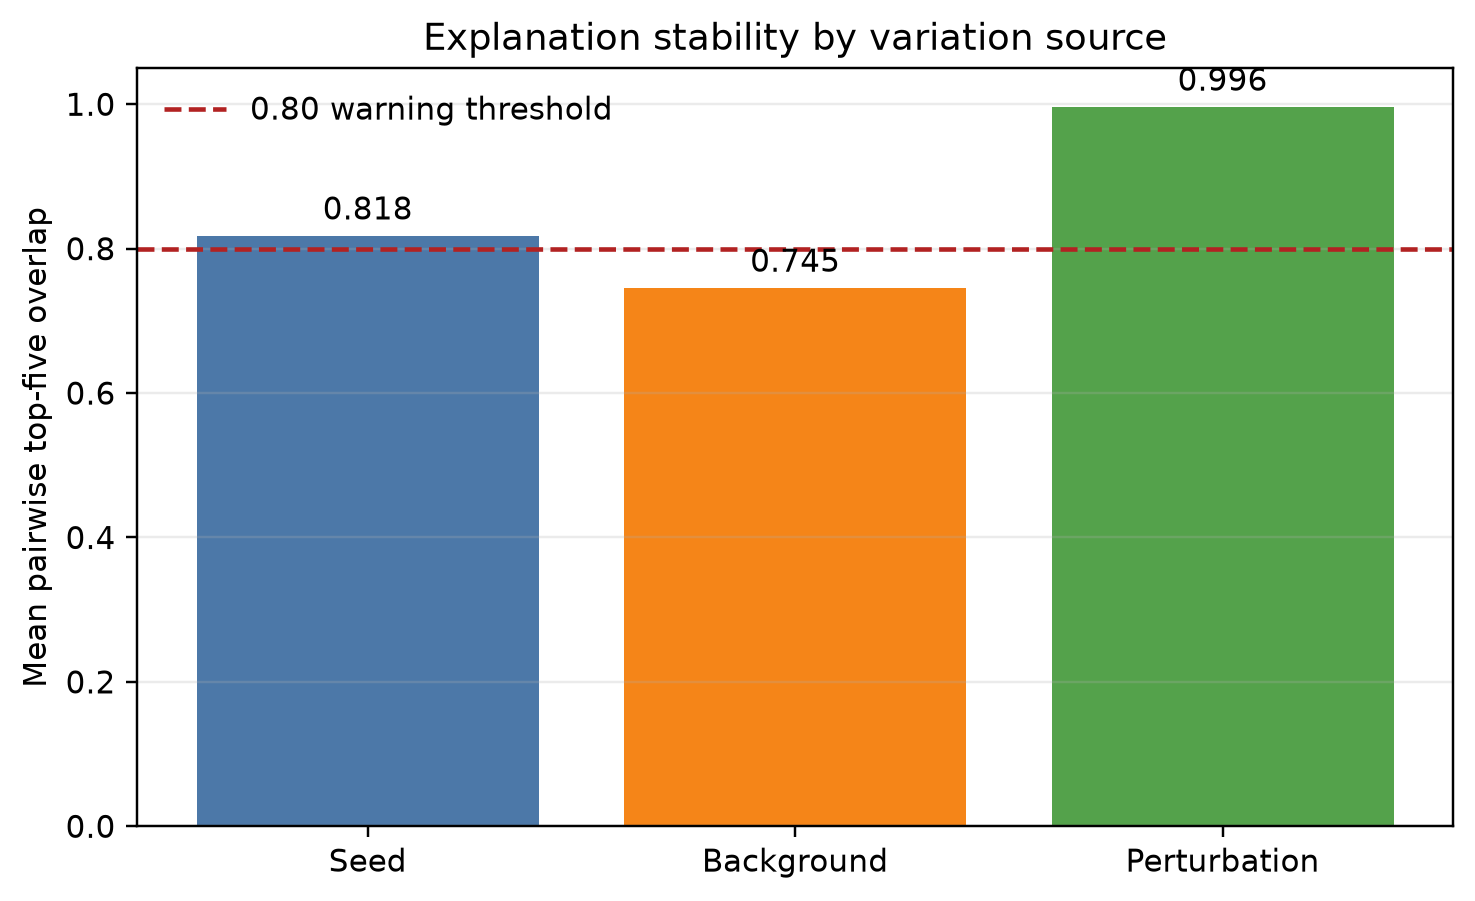
\includegraphics[width=\linewidth]{explanation_stability.png}
  \caption{Top-five stability over 10 recomputations (dashed line: 0.80 warning level).}
  \label{fig:stability}
\end{figure}

\textbf{Recourse and additivity.} Only 17 of the 108 flagged students would leave the top 20\% if
their debt or fee status changed; for the remaining 91, no such administrative change exists. For
example, for validation student 174, recording the fees as paid and the debt as cleared lowers the
estimate from 0.996 to 0.689 and the cohort rank from 87 to 182, outside the 108 slots
(Appendix~\ref{sec:app-interface}). The
best local surrogate (lasso with pair terms) approximated \tabicl with a mean absolute error of 0.022
on held-out masking patterns, against 0.073 without pair terms: the model's local behaviour is
captured well only once pairwise interactions are included.

\textbf{Summing the bars.} SHAP contributions sum by construction to the prediction minus the
comparison-group average, so all grouped contributions reproduce the ranking exactly. Even the five
bars shown to participants separate flagged from unflagged students (AUC 0.97; 89 of 108 flags
recovered).

\subsection{Sensitivity Analyses}
\label{sec:sensitivity}

\textbf{Enrolled students.} The frozen model scores still-enrolled students between the two known
groups (median 0.354, compared with 0.064 for graduates and 0.990 for dropouts). When a validation
share of 119 enrolled students joins the cohort, they receive 7 of 132 flags (5\%) despite forming
18\% of the cohort; with the number of slots held at 108, three flags move to enrolled students and
dropout recall falls from 0.507 to 0.493. Whether these seven flags are correct remains
unknown.

\textbf{Eligibility.} Setting aside the 49 validation students who took no first-semester
evaluation (36 of them dropouts) and re-ranking the remaining 495 with the frozen model, the top 20\%
(99 students) still contained only dropouts (precision 1.000), recall rose to 0.559 and ROC-AUC was
0.949 (Appendix Table~\ref{tab:sensitivity}). The flag is therefore not merely detecting students
who had already stopped attending, although the 99 flagged students remain those with weak
first-semester results.

\textbf{Admission-time window.} Without first-semester results, the validation ROC-AUC of \tabicl
fell from 0.952 to 0.874 and capacity recall from 0.507 to 0.469 (precision 0.926), with similar
declines for all models; first-semester results thus carry most of the signal.

\textbf{Without protected attributes.} Refitting \tabicl without gender, nationality, age,
international status, displacement and special needs changed the validation ROC-AUC from 0.952 to
0.950, left recall and precision at 0.507 and 1.000, and retained 103 of the 108 flags (the five
students swapped in and the five swapped out were all dropouts). The gender recall gap narrowed from
0.19 (0.404 vs.\ 0.597) to 0.10 (0.455 vs.\ 0.553).

\subsection{Human-Study Quantitative Results}
\label{sec:human}

All 50 assigned participants consented and completed the study, and none were excluded, yielding
500 scored responses. Mean accuracy was 0.916 with profiles only and 0.900 with explanation charts
(Table~\ref{tab:human}), a difference of $-0.016$ (95\% interval $-0.060$ to 0.032; exploratory
permutation $p=0.61$; Hedges' $g=-0.19$). There is thus no evidence that the charts helped
participants predict the flag. Participants with charts were, however, somewhat more confident
($+0.21$ points on a 1--5 scale, 0.02 to 0.42; $p=0.055$), whereas self-reported time did not differ
clearly.

\begin{table}[!htb]
\centering
\caption{Participant-level results (25 per group; 95\% bootstrap intervals).}
\label{tab:human}
\footnotesize
\setlength{\tabcolsep}{3pt}
\begin{tabular}{@{}lccc@{}}
\toprule
 & \textbf{Profiles only} & \textbf{+ Charts} & \textbf{B $-$ A} \\
\midrule
Accuracy   & 0.916 & 0.900 & $-$0.016 [$-$0.060, 0.032] \\
Confidence (1--5) & 4.14 & 4.35 & $+$0.21 [0.02, 0.42] \\
Minutes (self-rep.) & 33.4 & 30.2 & $-$3.2 [$-$8.7, 2.0] \\
\bottomrule
\end{tabular}
\end{table}

Accuracy was high in both groups, since most profiles were easy to judge: flagged cases usually
showed no passed units. With charts, accuracy rose on flagged cases (0.968 to 0.992) and fell on
unflagged ones (0.864 to 0.808), the fall coming entirely from one case. Participants described themselves as students (23), staff or advisers (23,
a broad option) or other (4), with similar accuracy across roles. Nine of the ten cases had equal or higher accuracy with charts. The
exception, case C01, was not flagged, yet its chart showed several factors pushing risk upwards;
accuracy fell from 0.60 without the chart to 0.20 with it (Figure~\ref{fig:human-case}). The chart
shows contributions relative to a typical student rather than the cohort cut-off and thus invites
the inference that ``more concern means flagged''. Without C01, the difference becomes $+0.027$
($-0.013$ to 0.076); this post-hoc check shows that the overall result depends on a single case but
does not establish a benefit. In Group~B, 21 of 25 participants passed both chart-reading checks.

\begin{figure}[!htb]
  \centering
  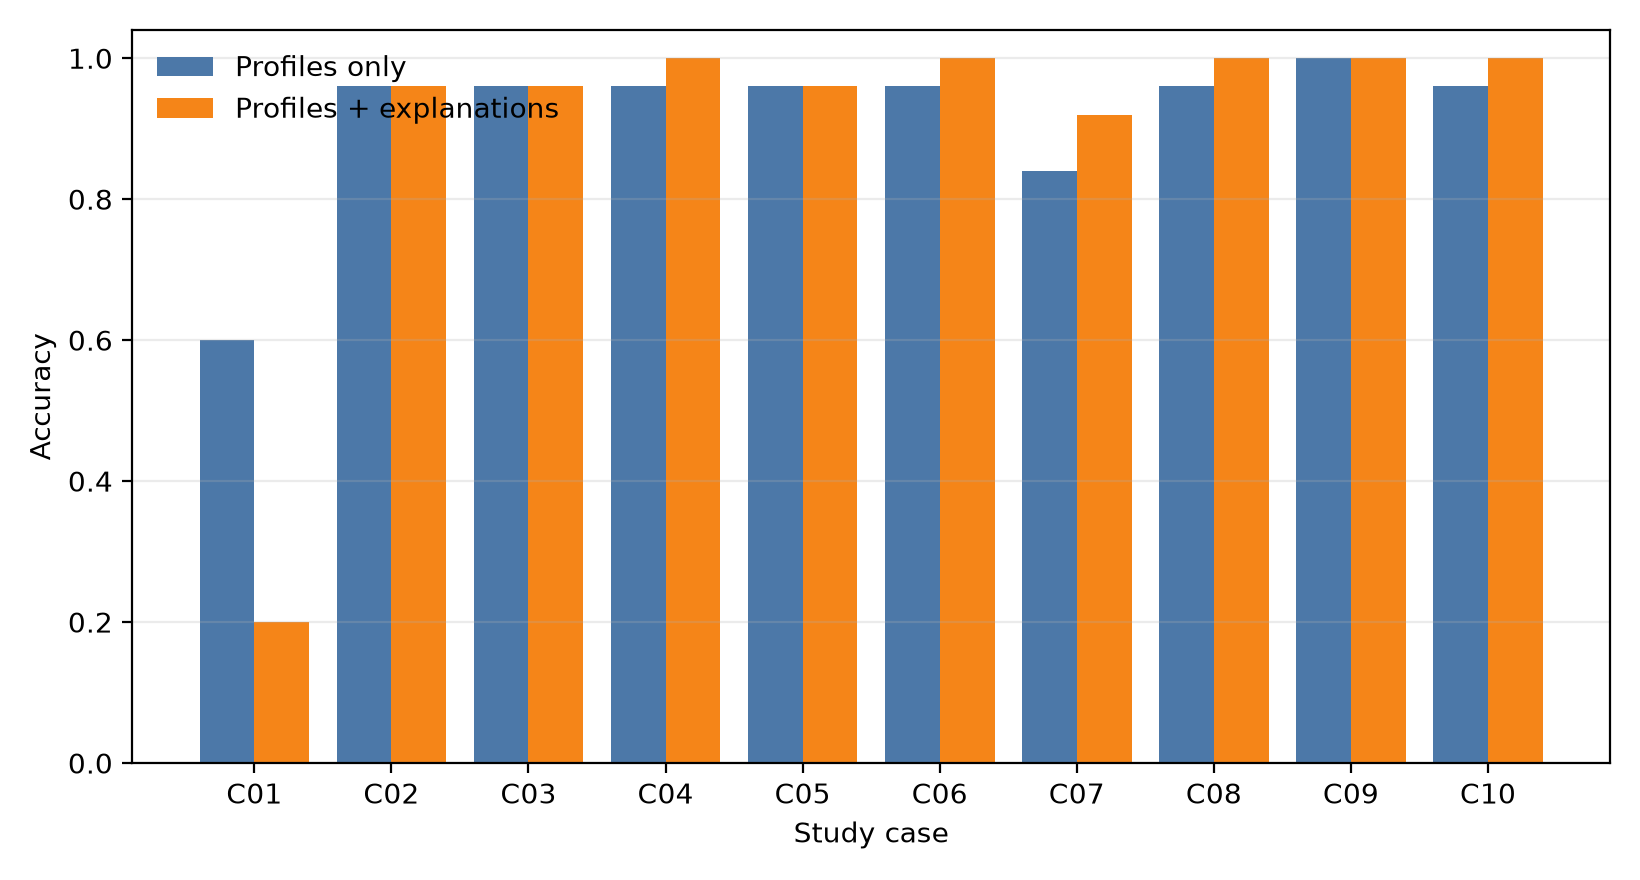
\includegraphics[width=\linewidth]{human_accuracy_by_case.png}
  \caption{Accuracy by case and group; C01 had lower accuracy with charts.}
  \label{fig:human-case}
\end{figure}

\subsection{Qualitative Findings}
\label{sec:qual}

The written answers are summarised from a single coding pass (Section~\ref{sec:methods}). When asked
why the model decided as it did, 72\% of chart-group answers reasoned from the chart, whereas the
profile-only group cited academic results (46\%) or several factors together (46\%); personal or
demographic reasons were almost never given (2 of 500). Suggested support was mostly academic
(30\%), followed by no action (21\%, mostly for unflagged students), advising or monitoring (16\%),
financial or administrative help (15\%) and first establishing what had happened (11\%); wellbeing
support was rare (2\%). Overall, 76\% of suggestions named a concrete next step (71\% without
charts and 82\% with them), 91\% could begin before the second semester and 2.8\% asserted an
unsupported cause. The chart group more often assigned the action to the institution (42\% vs.\
27\%). Asked what else they would want to know, participants most often named academic engagement,
such as attendance and current enrolment (40\%), and personal circumstances, such as work or family
(26\%), none of which the dataset contains. Typical answers, paraphrased, were that the long
first-semester bars pushed the estimate towards a flag; that the office should contact the student
about unpaid fees, offer a payment plan and then arrange tutoring; and that it would help to know
whether the student still attends and how many hours they work. The study was completed online, so
these are written comments rather than think-aloud remarks. Answer depth varied: some answers were generic, and 21
support suggestions matched another participant's answer word for word.
